% !TeX root = Bericht.tex
% !TeX spellcheck = de_DE
\section{Setup and procedure}
\begin{figure}[H]
	\centering
	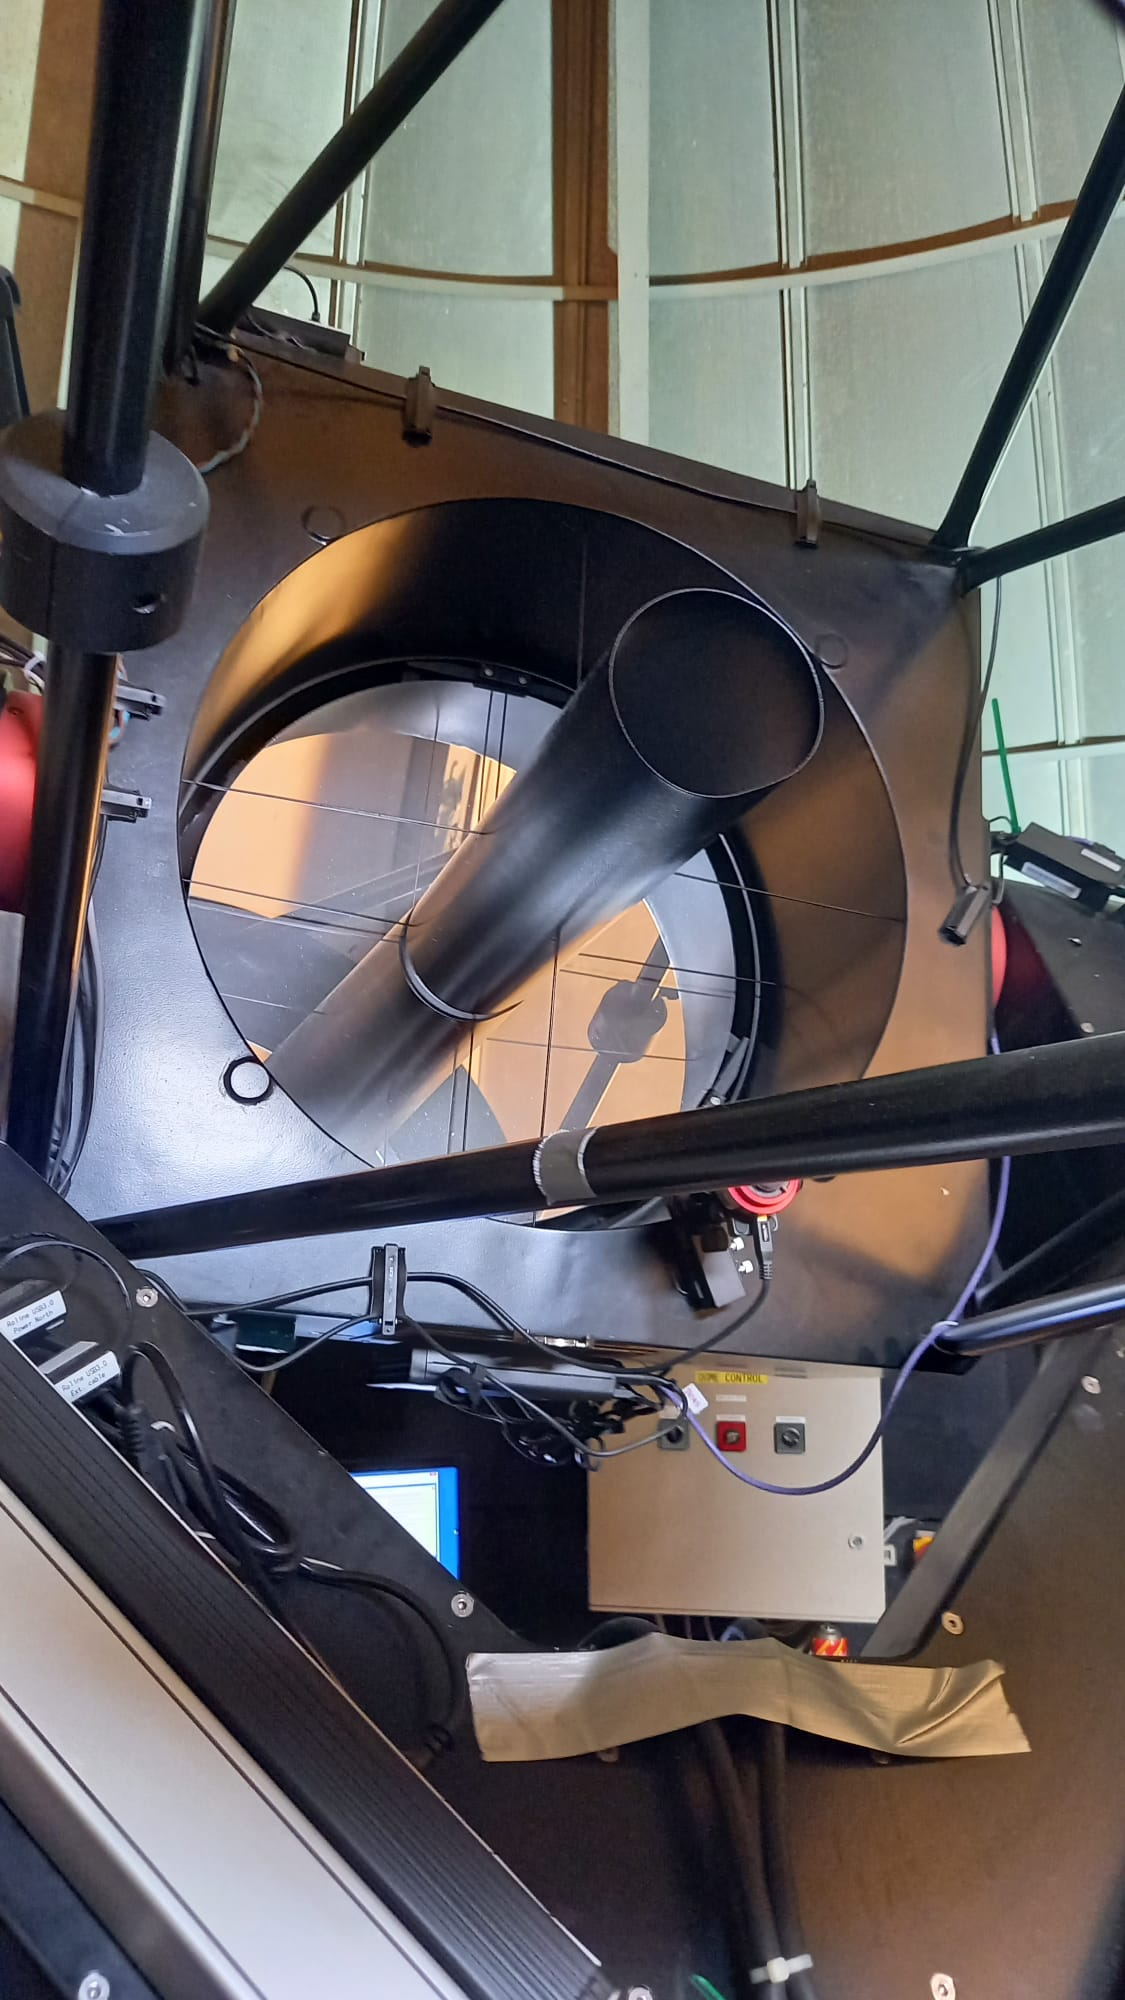
\includegraphics[width=0.8\linewidth,trim= 0 600 20 500,clip]{Bild Teleskop}
	\caption{The mirror of the thelescope with a diameter of 60cm can be seen, and the tube in which the light is focussed can also be seen.}
	\label{fig:teleskop}
\end{figure}


For the observations, the 60-cm-telescope on the roof of the Victor-Franz-Hess-building was used. To get a spectrum, an Echelle-spectrograph is connected to a telescope. The telescope can be seen in \autoref{fig:teleskop}.
Initially, the bias was measured, with 10 measurements taken at a length of 10 seconds. Subsequently, the flat field was measured, which is essential for characterising the pixel-to-pixel ratio. Subsequently, the measurement of the LAMP was taken with a measurement time of $0.1 \unit{s}$. These measurements were necessary to characterise the CCD. This enabled the actual spectrum of sunlight to be measured. For the final measurement, 10 measurements were taken with a length of $0.1\unit{ s}$. The time at this point was chosen to ensure a clear contrast.
The measured data enabled us to run the software to finally obtain the spectrum of sunlight. The final task was to identify the peaks and fit a Gaussian function to each. With this, it is possible to integrate the fitted function and finally obtain a spectrum with equivalent characteristics to the actual spectral lines, as well as the actual wavelength of the spectral lines. The corresponding wavelengths were provided and were derived from laboratory measurements of these specific samples. In \autoref{fit_gut}, an example of a fit with high quality is shown. Nevertheless, the data of absorption lines with bad fit quality should not be used. An example for such a fit is shown in \autoref{fit_schlecht}. Particular attention should be paid to peaks very close to each other. If they cannot be properly separated, the equivalent width of the two peaks is not calculated properly. Thus, both peaks are not used. 
\begin{figure}[H]
	\centering
	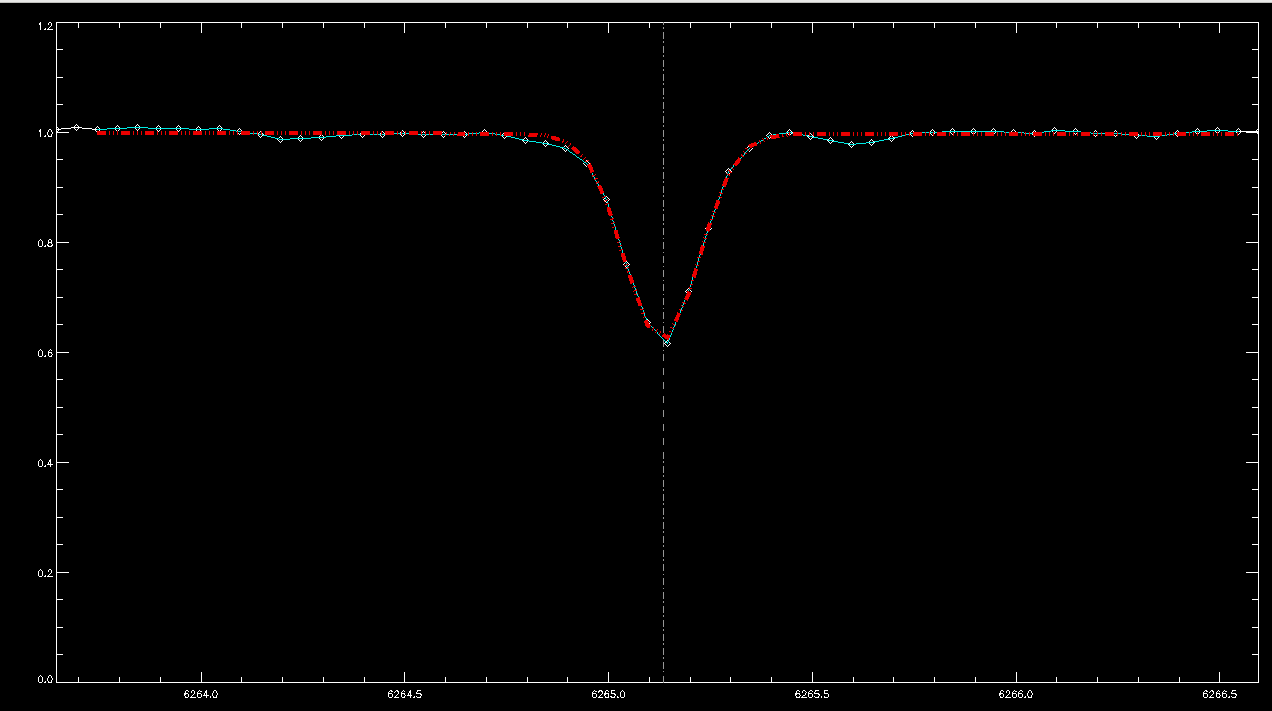
\includegraphics[width=0.6\linewidth]{screenshot_fit_gut}
	\caption{Example of a gaussian fit on an absorption line with high fit quality.}
	\label{fit_gut}
\end{figure}


\begin{figure}[H]
	\centering
	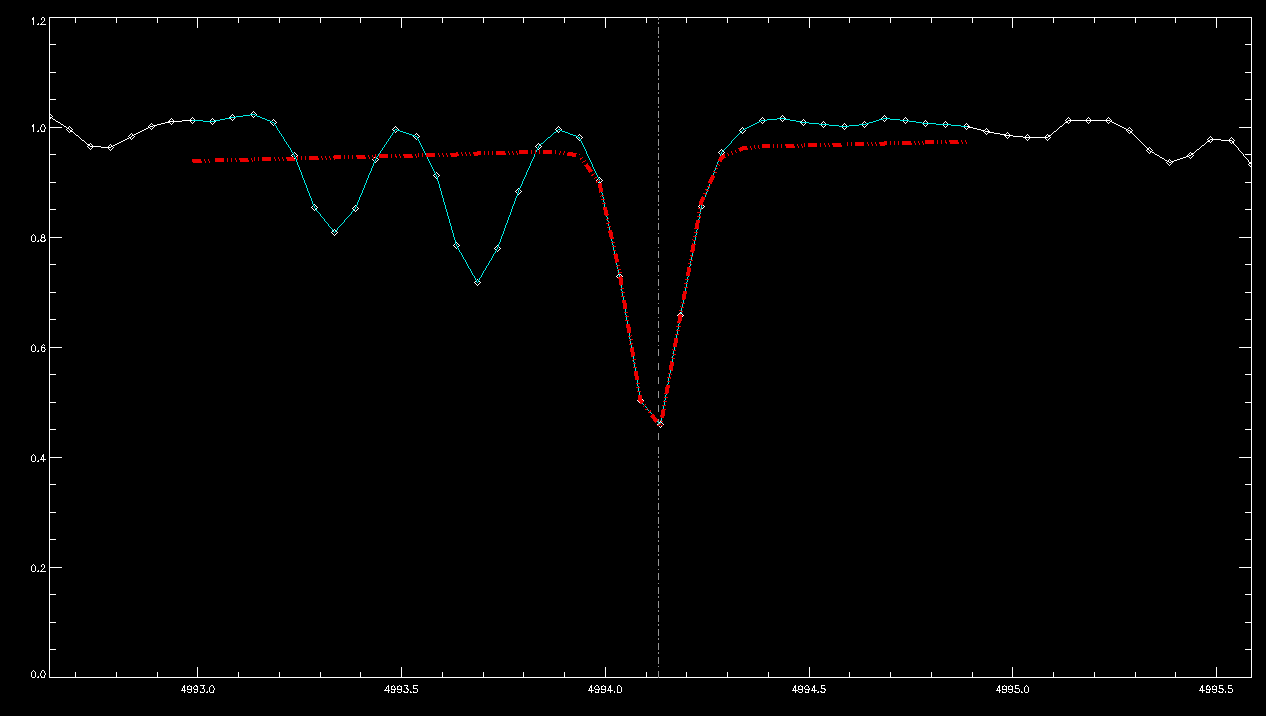
\includegraphics[width=0.6\linewidth]{screenshot_fit_schlecht}
	\caption{Example of a gaussian fit on an absorption line with low fit quality, which should not be used.}
	\label{fit_schlecht}
\end{figure}




%\begin{figure}[H]
%    \centering
%    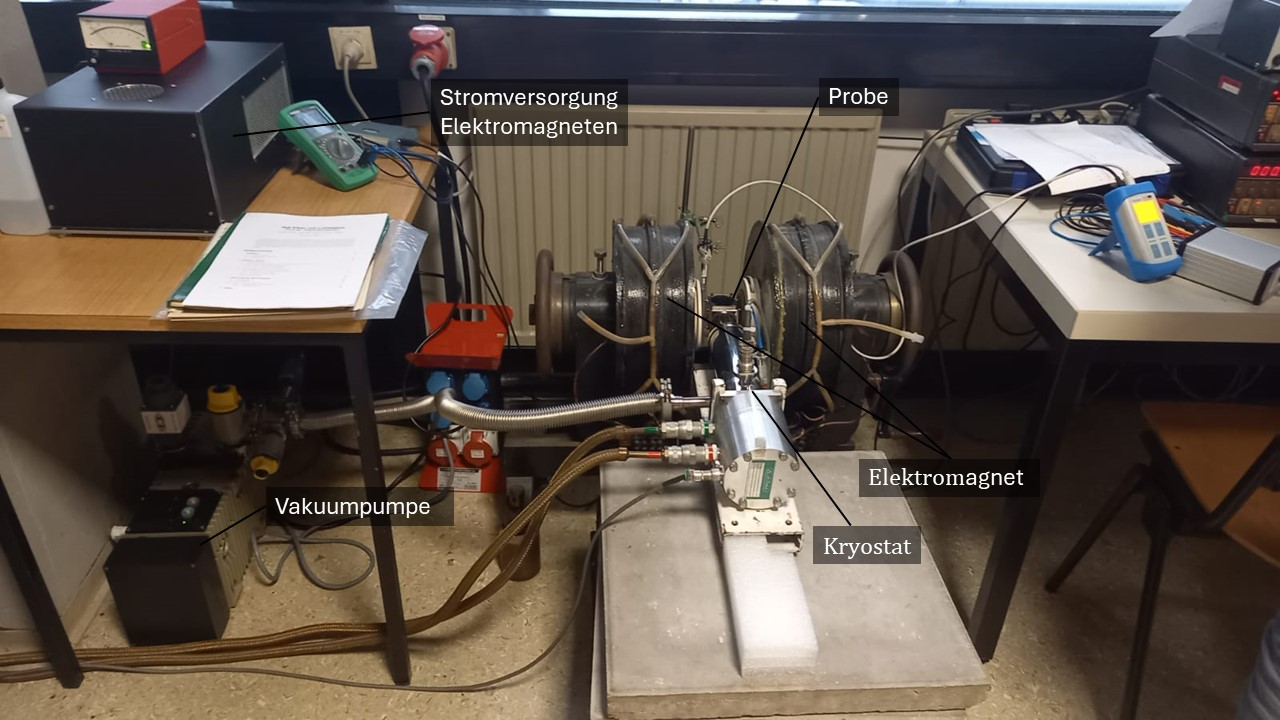
\includegraphics[width=\linewidth]{BildExberimentAufbauBeschriftung.JPG}
%    \caption{In dieser Abbildung sind der Kryostat, die Magnetspulen sowie die Sonde zur Messung des Magnetfeldes zu erkennen.}
%    \label{ExperimetAufbau}
%\end{figure}
